\section{Methode}

\subsection{Performance Test (Benchmarking)}
Unsere Performance Tests wurden mit der JUnit-Benchmark Bibliothek durchgeführt. Das ganze Programm sowie die grossen Teilschritte wurden geprüft. 

Die Tests wurden auf einem «HP Pavilion dv8 Notebook PC» durchgeführt. Das Gerät hat einen Intel i5 Prozessor mit 2.4GHz und vier Kernen. Dem Gerät stehen 8GB RAM zur Verfügung.


\subsection{Verzeichnisstruktur}
Da der OTP sehr viele verschiedene Pakete besitzt haben wir uns entschieden alles was den CSA betrifft und von uns programmiert wird in einem separaten Paket zu sammeln wie in Abbildung \ref{fig:csapackage} zu sehen. Dadurch behalten wir die Übersicht was wir zusätzlich in das bestehende Programm hinzugefügt haben. 

\begin{figure}[h]
	\centering
	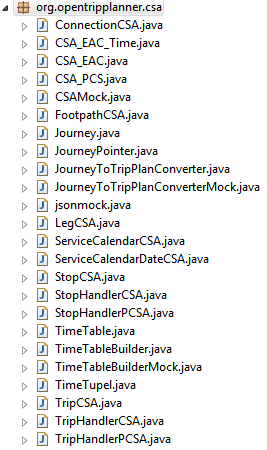
\includegraphics[width=5cm]{img/csapackage.png}
	\caption{Dieses Bild gibt eine Übersicht welche Klassen in unserem Paket vorhanden ist.}
	\label{fig:csapackage}
\end{figure}

Da ein Stop aus der Library gleich bei uns heissen würde. Führt dies zu einem Namenskonflikt mit der Klasse Stop für den CSA und Stop von der onebusaway Library. Ein weiterer Namenskonflikt war Leg diese Klasse ist schon im OTP(Grundversion) vorhanden.
Um dieses Problem zu lösen benannten wir die Klassen, die wir benötigen werden für den CSA um. Indem wir die Klassen mit der CSA Endung erweiterten z.B. Stop in StopCSA.\newline

\subsection{Zeitplan}
Für das Projekt wurde ein Zeitplan im Excel erstellt. Dann wurde jede Woche der «Ist» mit dem «Soll» zustand verglichen. Nach der Hälfte der Projektzeit stellten wir fest, dass wir für die Aufgaben durchgehend zu wenig Zeit eingeplant haben. Nach einer Absprache mit den Dozenten passten wir den Zeitplan entsprechend an. Das Reagieren auf Verspätungen wurde aus dem Scope entfernt und den anderen Teilaufgaben wurde mehr Zeit zugeteilt.
Zu einem späteren Zeitpunkt musste der Scope erneut aufgrund von erhöhtem Zeitaufwand angepasst werden. Die Fusswege zwischen den Stationen sowie die QuadTree-Optimierung wurden aus dem Scope entfernt.

\subsection{Mocking}
Das Programm kann grob in drei Abschnitte aufgeteilt werden. Das erstellen des Zeitplans aus den GTFS-Daten, den Wegfindungsalgorithmus und einen Converter welcher das Resultat in die von der Webseite verlangte Form bringt. Damit diese drei Abschnitte separat behandelt werden können und das Programm dennoch jederzeit überprüft werden kann entschieden wir uns ein Mockup für die Abschnitte durchzuführen.


